\section{Конструкторский раздел \hfill}
\vspace{\baselineskip}

В данном разделе приведены разработанные алгоритмы решения задачи коммивояжера: алгоритм полного перебора и муравьиный алгоритм.

\vspace{\baselineskip}
\subsection{Разработка алгоритмов} 
\vspace{\baselineskip}

На рисунке \ref{fig:full} приведена схема алгоритма полного перебора для решения задачи коммивояжера, а на рисунках \ref{fig:ant}--\ref{fig:ant3} --- схема муравьиного алгоритма.

\begin{figure}[h!btp]
	\centering
	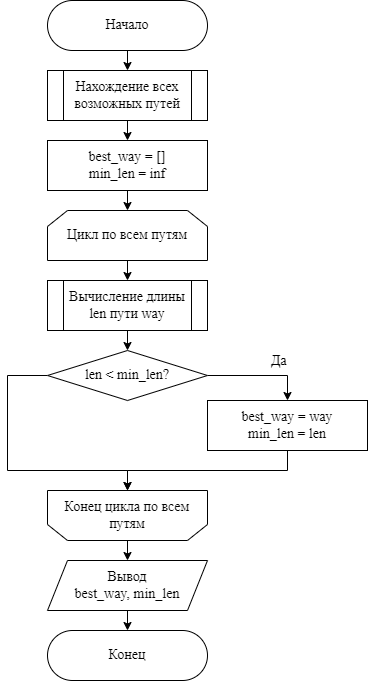
\includegraphics[width=240pt]{inc/scheme_full_search.png}
	\caption{Схема алгоритма полного перебора}
	\label{fig:full}	
\end{figure}

\clearpage

\begin{figure}[h!btp]
	\centering
	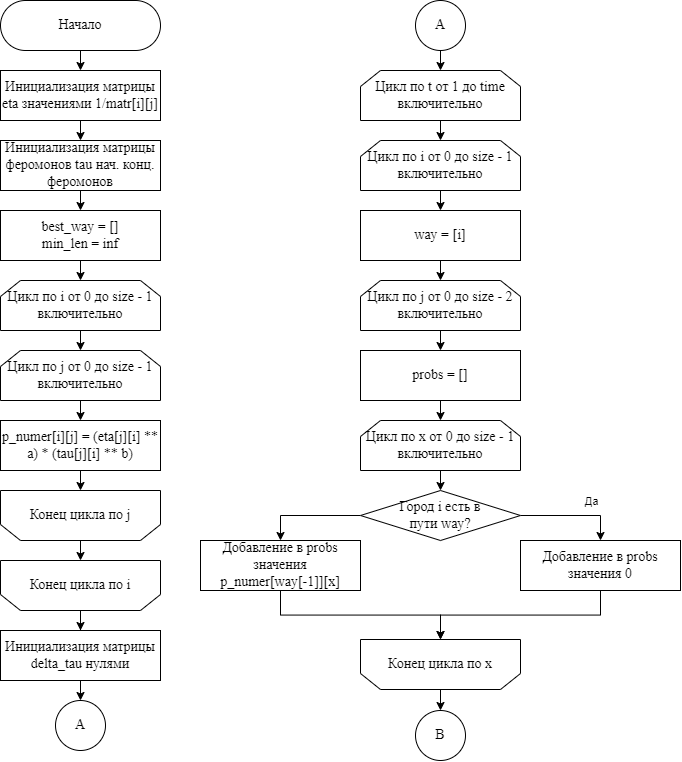
\includegraphics[width=420pt]{inc/scheme_ant_alg.png}
	\caption{Схема муравьиного алгоритма}
	\label{fig:ant}	
\end{figure}

\clearpage

\begin{figure}[h!btp]
	\centering
	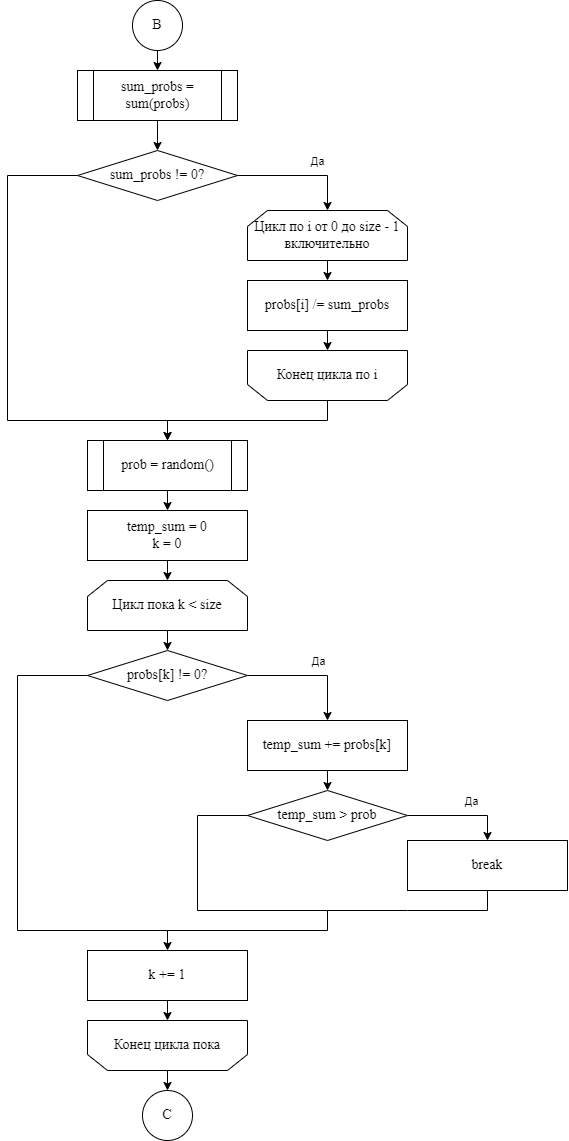
\includegraphics[width=340pt]{inc/scheme_ant_alg_2.png}
	\caption{Схема муравьиного алгоритма (продолжение)}
	\label{fig:ant2}	
\end{figure}

\clearpage

\begin{figure}[h!btp]
	\centering
	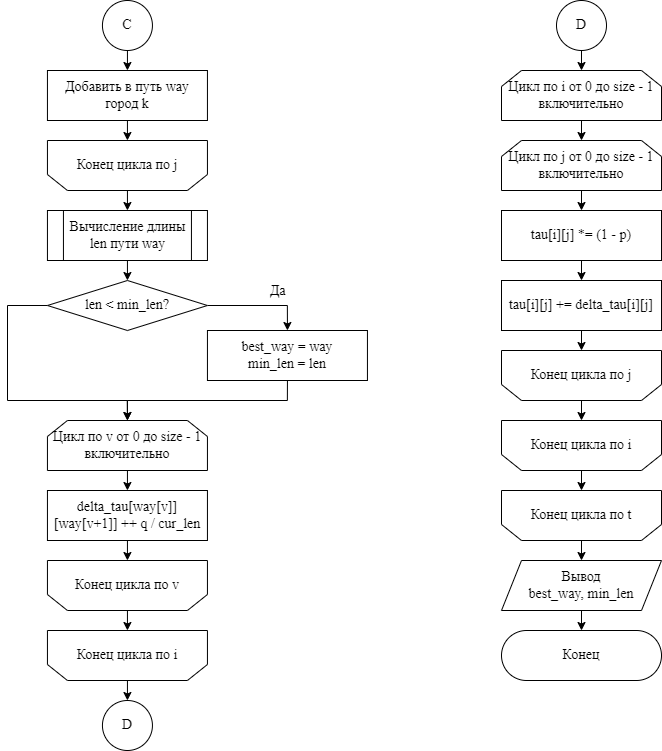
\includegraphics[width=400pt]{inc/scheme_ant_alg_3.png}
	\caption{Схема муравьиного алгоритма (продолжение)}
	\label{fig:ant3}	
\end{figure}

\vspace{\baselineskip}
\subsection{Требования к программному обеспечению}
\vspace{\baselineskip}

Программа должна предоставлять следующие возможности:
\begin{itemize}[label=---]
    \item выбор файла с матрицей расстояний;
    \item ввод параметров $\alpha$, $p$ и $t_{max}$ для муравьиного алгоритма;
    \item вывод на экран найденного каждым из алгоритмов кратчайшего пути и его длины;
    \item измерение времени работы реализаций алгоритмов на матрицах разных размеров и представление результата в виде графика;
    \item вывод результатов параметризации муравьиного алгоритма в текстовый файл.
\end{itemize}

\vspace{\baselineskip}
\subsection*{Вывод}
\vspace{\baselineskip}

Были разработаны алгоритмы для решения задачи коммивояжера: алгоритм полного перебора и муравьиный алгоритм.
